\documentclass[a4paper,fleqn]{cas-dc}

%%%Author definitions
\def\tsc#1{\csdef{#1}{\textsc{\lowercase{#1}}\xspace}}
\tsc{WGM}
\tsc{QE}
\tsc{EP}
\tsc{PMS}
\tsc{BEC}
\tsc{DE}
%%%

\usepackage[square,numbers,sort&compress,comma]{natbib}

\usepackage{amsmath}
\usepackage{amssymb}
\usepackage{diagbox}
\usepackage{caption}
\usepackage{graphicx}
\usepackage{latexsym}
\usepackage{times}
\usepackage[pagewise]{lineno}
\graphicspath{{figures/}}
\usepackage{color, colortbl}
\usepackage{chemformula}
\usepackage{xcolor}
\definecolor{Gray}{gray}{0.9}
\newcommand{\highlight}[1]{%
  \colorbox{Gray}{$\displaystyle#1$}}
\usepackage{color, colortbl}
\usepackage{chemformula}
\usepackage{xcolor}
\usepackage{adjustbox}
\usepackage{mathrsfs}
\usepackage{booktabs}
\usepackage{hyperref}
\usepackage{lipsum}

\emergencystretch = 0 pt
\pretolerance = 150
\tolerance = 250
\hbadness = 150
\hfuzz = 0 pt
\vfuzz = 0 pt

\newcommand{ \kamila}[1]{\color{blue}{Kamila: #1} \color{black}}
\newcommand{ \todump}[1]{\color{olive}{#1} \color{black}}
\usepackage[normalem]{ulem}

\begin{document}

\shorttitle{\texttt{pykitPIV}: PyTorch-compatible synthetic image generation for training flow estimation algorithms in particle image velocimetry}
\shortauthors{Zdyba\l{} et~al.}


\title [mode = title]{\texttt{pykitPIV}: PyTorch-compatible synthetic image generation for training flow estimation algorithms in particle image velocimetry}

\author[EMPA]{Kamila Zdyba\l{}*}
\ead{kamila.zdybal@gmail.com}

\author[EMPA]{Claudio Mucignat}
\author[EMPA]{Ivan Lunati}

\address[EMPA]{Laboratory for Computational Engineering, Swiss Federal Laboratories for Materials Science and Technology, Empa, Dübendorf, Switzerland}

\begin{abstract} 
We describe \texttt{pykitPIV}, a PyTorch-compatible Python library for generating synthetic images that mimic those obtained from particle image velocimetry (PIV) experiments. The library can be readily ported to training machine learning algorithms, such as convolutional neural networks (CNNs), or reinforcement learning (RL). Our image generation exploits the kinematic relationship between two PIV snapshots and advects particles from one time frame at $t_1$, to the next at $t_1 + \Delta t$, with a second-order accurate numerical scheme. This results in paired image intensities, $I_1$ and $I_2$ that are separated by $\Delta t$ in time. The goal of this library is to give the user a lot of flexibility in selecting various parameters that would normally be available in an experimental setting such as particle seeding density, thickness of the laser plane, camera exposure, particle loss due to out-of-plane movement, or $\Delta t$ between images. The richness of image generation can help answer outstanding questions in training CNNs or RL algorithms.
\end{abstract}

\begin{keywords}
particle image velocimetry; flow estimation; convolutional neural networks; machine learning; Python; PyTorch
\end{keywords}

\maketitle

\section{Introduction\label{sec:introduction}}

The last decade has seen many advances in training convolutional neural networks (CNNs) for flow estimation, \textit{i.e.}, predicting motion information from consecutive static image frames. To date, numerous interesting network architectures have been developed, along with general advancements in training case-specific CNNs. This includes various implementations of FlowNets \citep{dosovitskiy2015flownet, ilg2017flownet, hui2018liteflownet}, spatial pyramid network (SPyNet) \cite{ranjan2017optical}, pyramid, warping and cost-volume network (PWC-Net) \cite{sun2018pwc}, and recurrent all-pairs field transforms (RAFT) \cite{teed2020raft}. In addition, the idea of the iterative residual refinement (IRR) \cite{hur2019iterative} allowed for significant reduction in the number of trainable parameters thanks to weight-sharing at several levels of successively upscaling image resolution.

Particle image velocimetry (PIV) can especially profit from those architectures, since its main goal is to predict flow targets, such as velocity components, velocity magnitude, or vorticity, from paired snapshots of illuminated tracer particles injected into the flow. Recently, RAFT-PIV \cite{lagemann2021deep} and lightweight image-matching architecture (LIMA) \citep{manickathan2023lightweight} were proposed as versions of CNNs that are specifically optimized for predicting flow targets from velocimetry experiments. Thanks to this targeted optimization of CNN architecture and training parameters, both RAFT-PIV and LIMA achieve high accuracy and per-pixel resolution and LIMA is significantly lighter than its predecessors.

The successes of RAFT-PIV and LIMA has been demonstrated on a number of classic experimental fluid dynamics settings such as flow behind a cylinder or boundary layer flow.
However, to advance the accuracy of training CNNs for more complex PIV applications, a number of research questions will have to be addressed next:
\begin{enumerate}
\item How rich does the training dataset need to be to remain applicable in a given experimental setting?
\item What degree of data augmentation is sufficient to transfer knowledge from one trained CNN to the next when changing experimental settings?
\item At what time separation, $\Delta t$, would the current CNN architectures fail?
\end{enumerate}


To help researchers answer those questions, we propose the present Python library \texttt{pykitPIV} -- \textbf{Py}thon \textbf{ki}nematic \textbf{t}raining for \textbf{PIV}. Our library is compatible with PyTorch \cite{paszke2017automatic, paszke2019pytorch} to allow for easier porting with machine learning algorithms.




\section{Software overview} \label{sec:software}

All functionalities of \texttt{pykitPIV} are organized in five classes.
Fig.~\ref{fig:pykitPIV-overview} illustrates the hierarchy of using \texttt{pykitPIV} classes and briefly describes what can be achieved with each class.

\begin{figure*}[t]
\centering
\vspace{-0.4 in}
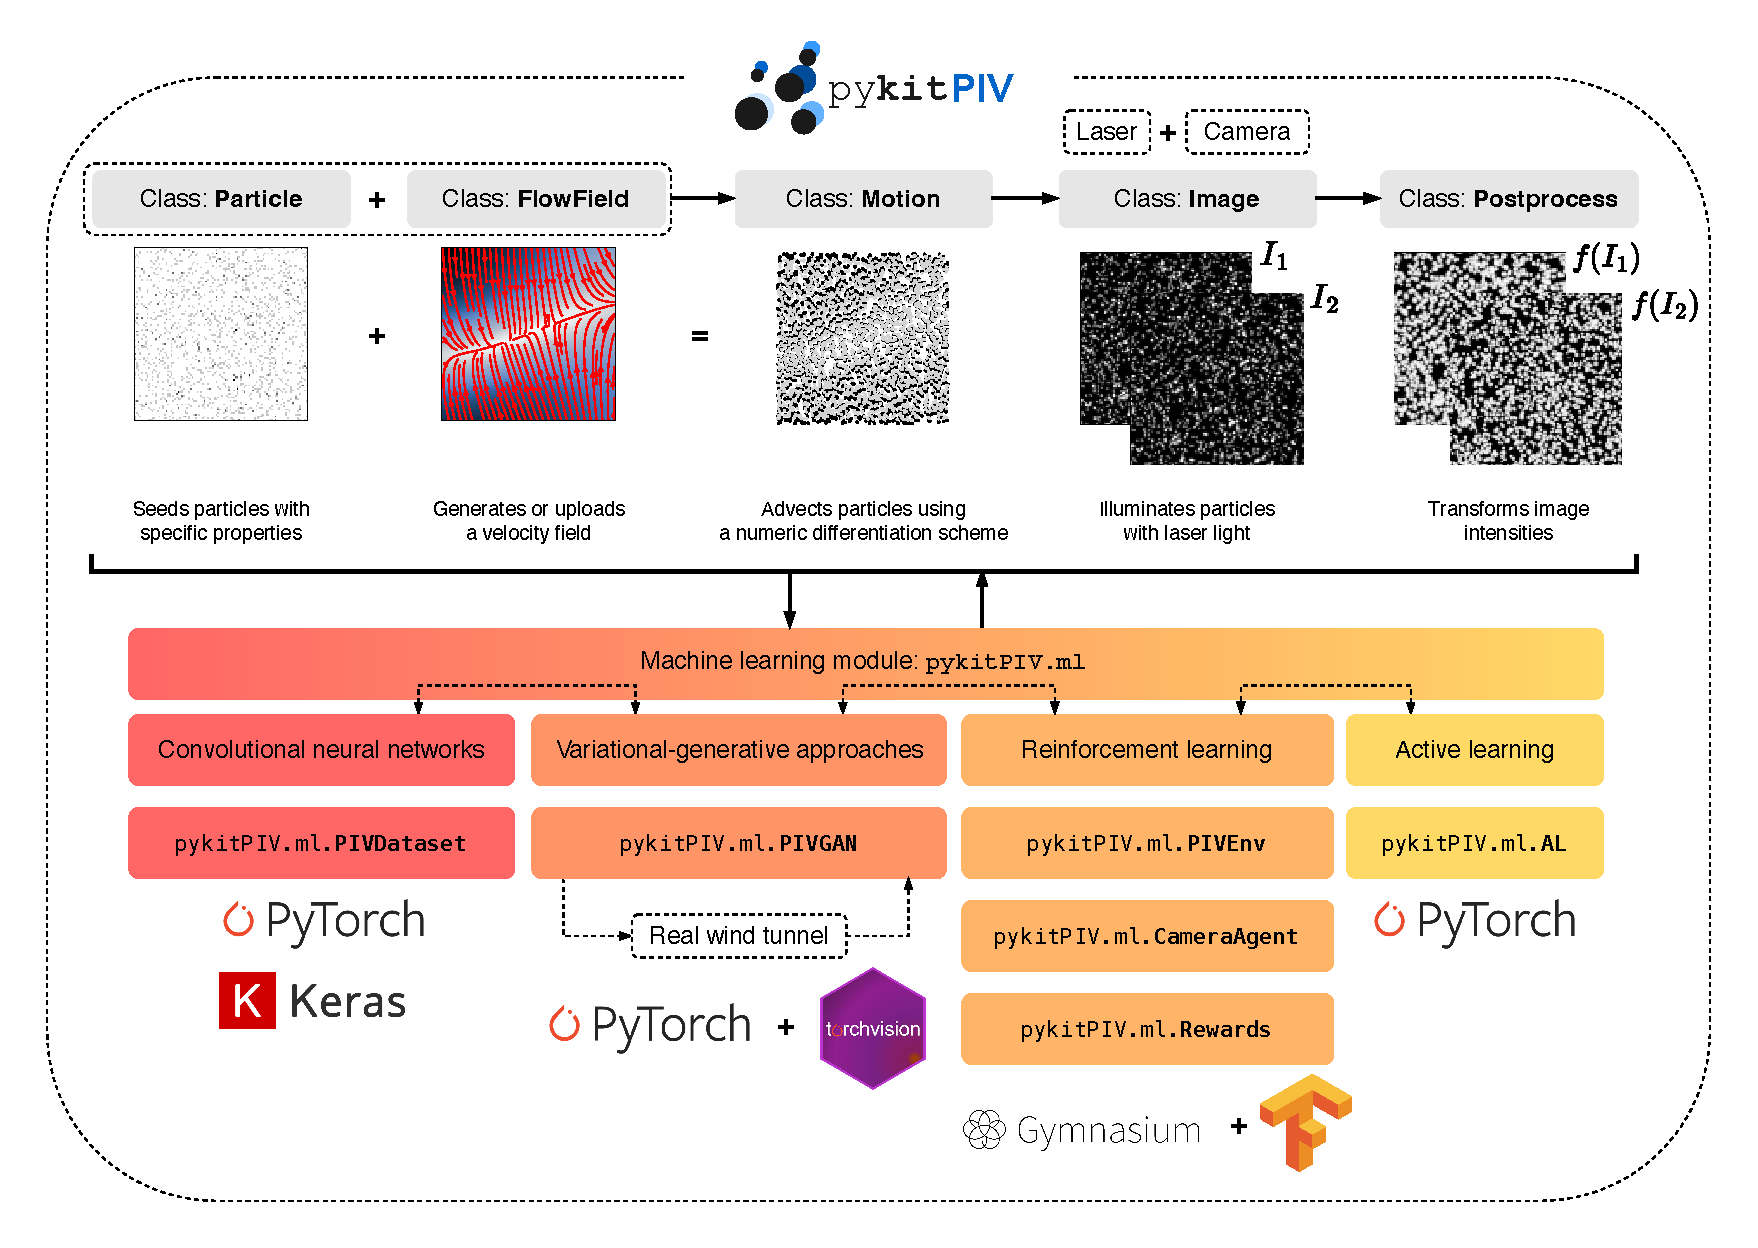
\includegraphics[width=\textwidth]{pykitPIV-modules.pdf}
\vspace{10 pt}
\caption{\footnotesize Order of using \texttt{pykitPIV} classes. At each stage of synthetic image generation, the user has freedom in selecting various parameters that would normally be available in an experimental setting such as particle seeding density, thickness of the laser plane, camera exposure, particle loss due to out-of-plane movement, or time separation between images.}
\label{fig:pykitPIV-overview}
\end{figure*}

\subsection{Class: \texttt{Particle}} \label{sec:class-Particle}

The \texttt{Particle} class seeds the two-dimensional flow domain with particles. The user can steer the range of particle diameters and the seeding density.


\subsection{Class: \texttt{FlowField}} \label{sec:class-FlowField}

The \texttt{FlowField} class allows to generate the velocity field to be applied on the two-dimensional domain. We implemented several methods to generate velocity fields, such as random smooth field, checkered field, Chebyshev polynomial field, or simple harmonics field. Those are illustratively visualized in Fig.~\ref{fig:velocity-fields}a-d. This variety of velocity fields span cases with smooth and sharp velocity gradients and can help put machine learning algorithms to test.

The user also has the option of uploading an external velocity field, \textit{e.g.}, coming from numerical simulation of Navier-Stokes equations (\textit{cf.} Fig.~\ref{fig:velocity-fields}e), or coming from a synthetic turbulence generator (\textit{cf.} Fig.~\ref{fig:velocity-fields}f).

\begin{figure}[t]
\centering
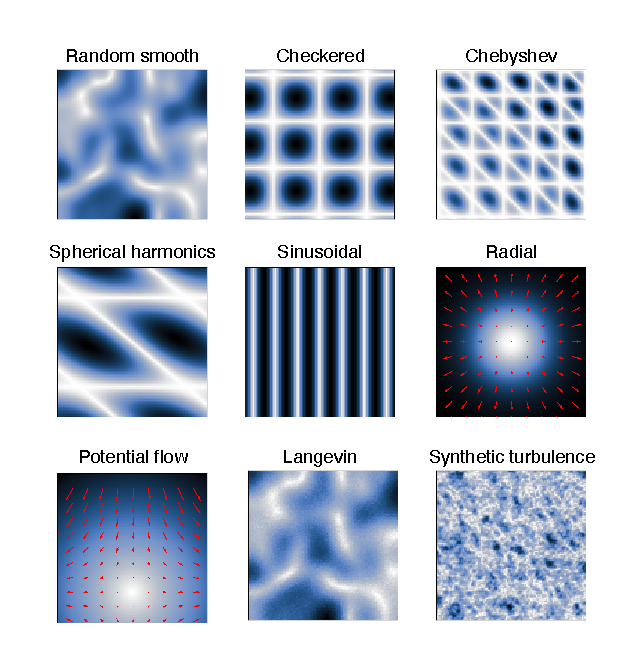
\includegraphics[width=9cm]{velocity-fields.pdf}
\caption{Types of two-dimensional velocity fields that can be generated with or uploaded to the \texttt{FlowField} class.}
\label{fig:velocity-fields}
\end{figure}

\subsection{Class: \texttt{Motion}} \label{sec:class-Motion}

The \texttt{Motion} class applies the flow field to the particles. It uses RK-4 numeric scheme to advect particles by a user-specified time separation, $\Delta t$. The main output of this class are paired PIV images, $I_1$ and $I_2$.

\subsection{Class: \texttt{Image}} \label{sec:class-Image}

The \texttt{Image} class helps generate image intensities. It adds the reflected laser light to the generated image pairs. The core functionality is to add Gaussian intensity to each particle. The user has a lot of flexibility in setting up the laser plane and camera properties. The user can also steer the amount of particles lost between frame $I_1$ and $I_2$ due to out-of-plane movement.

The PIV image pair tensor has shape $(N, 2, H, W)$, where $N$ is the batch size, $H$ is image height and $W$ is image width. The second dimension can be thought of as the number of channels and those correspond to $I_1$ and $I_2$, respectively. This is compatible with tensor shape accepted by convolutional layers implemented in PyTorch. Note that the user can generate a whole batch, $N$, of images all at once. The \texttt{Image} class contains convenient functions for saving images to \texttt{.h5} files and for plotting or animating image pairs. \texttt{pykitPIV} uses sequential colormaps by Crameri et al. \cite{crameri2020misuse}.

\subsection{Class: \texttt{Postprocess}} \label{sec:class-Postprocess}

The \texttt{Postprocess} class contains functions that apply transformations to generated images. It can be especially useful for data augmentation.

\section{Discussion} \label{sec:results}

%
%\begin{figure*}[t]
%\centering
%\vspace{-0.4 in}
%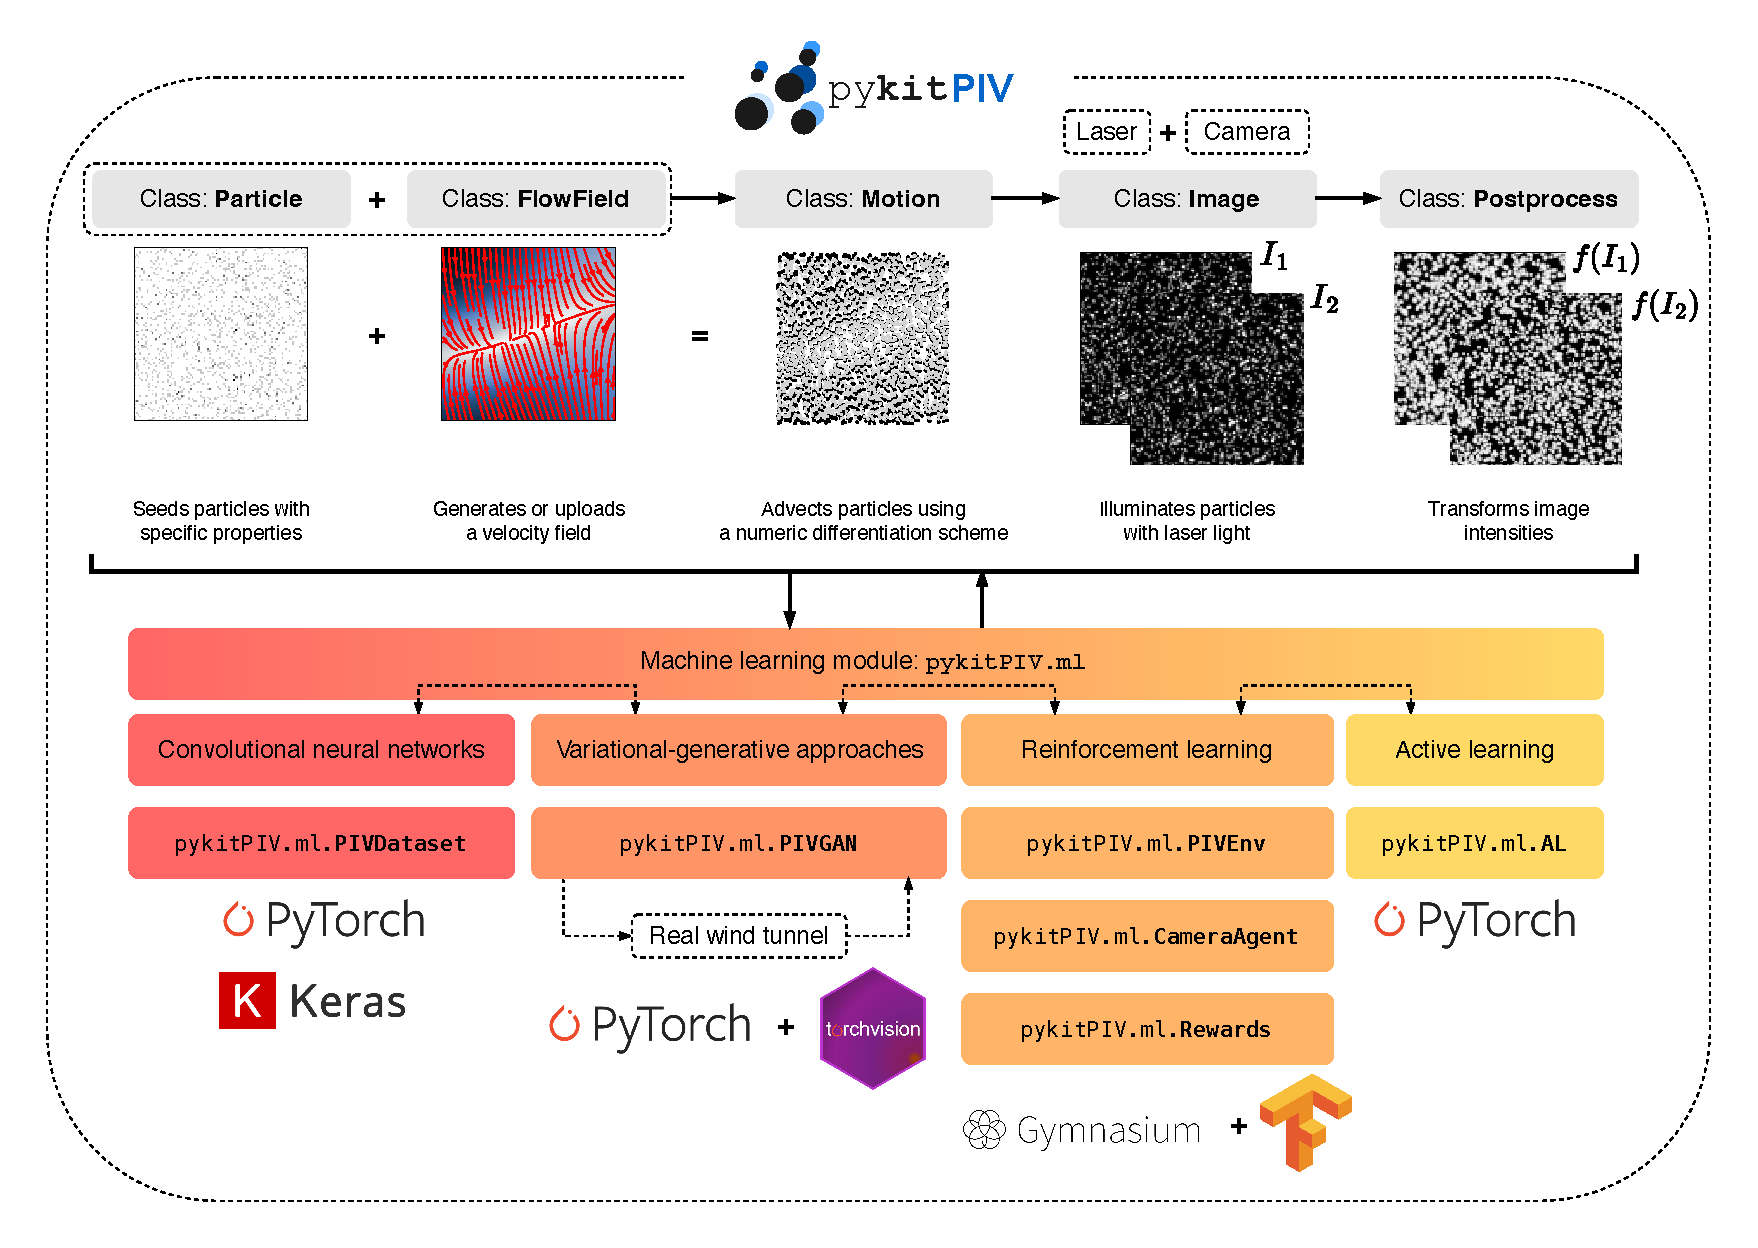
\includegraphics[width=\textwidth]{pykitPIV-modules.pdf}
%\vspace{10 pt}
%\caption{\footnotesize The variety of operations on PIV images possible with the pykitPIV modules.}
%\label{fig:operations}
%\end{figure*}

\section{Conclusions}



\section*{Declaration of competing interest}

The authors declare that they have no known competing financial interests or personal relationships that could have appeared to influence the work reported in this paper.

\section*{Author contributions}



\section*{Acknowledgments}




\bibliographystyle{pci}
\bibliography{bibliography}

\end{document}